\documentclass[twoside]{book}

% Packages required by doxygen
\usepackage{fixltx2e}
\usepackage{calc}
\usepackage{doxygen}
\usepackage[export]{adjustbox} % also loads graphicx
\usepackage{graphicx}
\usepackage[utf8]{inputenc}
\usepackage{makeidx}
\usepackage{multicol}
\usepackage{multirow}
\PassOptionsToPackage{warn}{textcomp}
\usepackage{textcomp}
\usepackage[nointegrals]{wasysym}
\usepackage[table]{xcolor}

% Font selection
\usepackage[T1]{fontenc}
\usepackage[scaled=.90]{helvet}
\usepackage{courier}
\usepackage{amssymb}
\usepackage{sectsty}
\renewcommand{\familydefault}{\sfdefault}
\allsectionsfont{%
  \fontseries{bc}\selectfont%
  \color{darkgray}%
}
\renewcommand{\DoxyLabelFont}{%
  \fontseries{bc}\selectfont%
  \color{darkgray}%
}
\newcommand{\+}{\discretionary{\mbox{\scriptsize$\hookleftarrow$}}{}{}}

% Page & text layout
\usepackage{geometry}
\geometry{%
  a4paper,%
  top=2.5cm,%
  bottom=2.5cm,%
  left=2.5cm,%
  right=2.5cm%
}
\tolerance=750
\hfuzz=15pt
\hbadness=750
\setlength{\emergencystretch}{15pt}
\setlength{\parindent}{0cm}
\setlength{\parskip}{3ex plus 2ex minus 2ex}
\makeatletter
\renewcommand{\paragraph}{%
  \@startsection{paragraph}{4}{0ex}{-1.0ex}{1.0ex}{%
    \normalfont\normalsize\bfseries\SS@parafont%
  }%
}
\renewcommand{\subparagraph}{%
  \@startsection{subparagraph}{5}{0ex}{-1.0ex}{1.0ex}{%
    \normalfont\normalsize\bfseries\SS@subparafont%
  }%
}
\makeatother

% Headers & footers
\usepackage{fancyhdr}
\pagestyle{fancyplain}
\fancyhead[LE]{\fancyplain{}{\bfseries\thepage}}
\fancyhead[CE]{\fancyplain{}{}}
\fancyhead[RE]{\fancyplain{}{\bfseries\leftmark}}
\fancyhead[LO]{\fancyplain{}{\bfseries\rightmark}}
\fancyhead[CO]{\fancyplain{}{}}
\fancyhead[RO]{\fancyplain{}{\bfseries\thepage}}
\fancyfoot[LE]{\fancyplain{}{}}
\fancyfoot[CE]{\fancyplain{}{}}
\fancyfoot[RE]{\fancyplain{}{\bfseries\scriptsize Generated by Doxygen }}
\fancyfoot[LO]{\fancyplain{}{\bfseries\scriptsize Generated by Doxygen }}
\fancyfoot[CO]{\fancyplain{}{}}
\fancyfoot[RO]{\fancyplain{}{}}
\renewcommand{\footrulewidth}{0.4pt}
\renewcommand{\chaptermark}[1]{%
  \markboth{#1}{}%
}
\renewcommand{\sectionmark}[1]{%
  \markright{\thesection\ #1}%
}

% Indices & bibliography
\usepackage{natbib}
\usepackage[titles]{tocloft}
\setcounter{tocdepth}{3}
\setcounter{secnumdepth}{5}
\makeindex

% Hyperlinks (required, but should be loaded last)
\usepackage{ifpdf}
\ifpdf
  \usepackage[pdftex,pagebackref=true]{hyperref}
\else
  \usepackage[ps2pdf,pagebackref=true]{hyperref}
\fi
\hypersetup{%
  colorlinks=true,%
  linkcolor=blue,%
  citecolor=blue,%
  unicode%
}

% Custom commands
\newcommand{\clearemptydoublepage}{%
  \newpage{\pagestyle{empty}\cleardoublepage}%
}

\usepackage{caption}
\captionsetup{labelsep=space,justification=centering,font={bf},singlelinecheck=off,skip=4pt,position=top}

%===== C O N T E N T S =====

\begin{document}

% Titlepage & ToC
\hypersetup{pageanchor=false,
             bookmarksnumbered=true,
             pdfencoding=unicode
            }
\pagenumbering{alph}
\begin{titlepage}
\vspace*{7cm}
\begin{center}%
{\Large cpu\+Information }\\
\vspace*{1cm}
{\large Generated by Doxygen 1.8.13}\\
\end{center}
\end{titlepage}
\clearemptydoublepage
\pagenumbering{roman}
\tableofcontents
\clearemptydoublepage
\pagenumbering{arabic}
\hypersetup{pageanchor=true}

%--- Begin generated contents ---
\chapter{Hierarchical Index}
\section{Class Hierarchy}
This inheritance list is sorted roughly, but not completely, alphabetically\+:\begin{DoxyCompactList}
\item Q\+Abstract\+List\+Model\begin{DoxyCompactList}
\item \contentsline{section}{C\+P\+U\+Model}{\pageref{class_c_p_u_model}}{}
\end{DoxyCompactList}
\end{DoxyCompactList}

\chapter{Class Index}
\section{Class List}
Here are the classes, structs, unions and interfaces with brief descriptions\+:\begin{DoxyCompactList}
\item\contentsline{section}{\hyperlink{class_c_p_u_model}{C\+P\+U\+Model} \\*The \hyperlink{class_c_p_u_model}{C\+P\+U\+Model} class This class contains the list model for processor information extracted from \textquotesingle{}/proc/cpuinfo\textquotesingle{} file in a Linux system. The class is derived from Q\+Abstract\+List\+Model }{\pageref{class_c_p_u_model}}{}
\end{DoxyCompactList}

\chapter{File Index}
\section{File List}
Here is a list of all files with brief descriptions\+:\begin{DoxyCompactList}
\item\contentsline{section}{C\+:/\+Users/\+S\+H\+E\+K\+H\+A\+R/\+Desktop/\+C\+P\+U\+\_\+\+Info/cpu\+Information/\hyperlink{cpumodel_8cpp}{cpumodel.\+cpp} }{\pageref{cpumodel_8cpp}}{}
\item\contentsline{section}{C\+:/\+Users/\+S\+H\+E\+K\+H\+A\+R/\+Desktop/\+C\+P\+U\+\_\+\+Info/cpu\+Information/\hyperlink{cpumodel_8h}{cpumodel.\+h} }{\pageref{cpumodel_8h}}{}
\item\contentsline{section}{C\+:/\+Users/\+S\+H\+E\+K\+H\+A\+R/\+Desktop/\+C\+P\+U\+\_\+\+Info/cpu\+Information/\hyperlink{globalconstants_8h}{globalconstants.\+h} }{\pageref{globalconstants_8h}}{}
\item\contentsline{section}{C\+:/\+Users/\+S\+H\+E\+K\+H\+A\+R/\+Desktop/\+C\+P\+U\+\_\+\+Info/cpu\+Information/\hyperlink{main_8cpp}{main.\+cpp} }{\pageref{main_8cpp}}{}
\end{DoxyCompactList}

\chapter{Class Documentation}
\hypertarget{class_c_p_u_model}{}\section{C\+P\+U\+Model Class Reference}
\label{class_c_p_u_model}\index{C\+P\+U\+Model@{C\+P\+U\+Model}}


The \hyperlink{class_c_p_u_model}{C\+P\+U\+Model} class This class contains the list model for processor information extracted from \textquotesingle{}/proc/cpuinfo\textquotesingle{} file in a Linux system. The class is derived from Q\+Abstract\+List\+Model.  




{\ttfamily \#include $<$cpumodel.\+h$>$}

Inheritance diagram for C\+P\+U\+Model\+:\begin{figure}[H]
\begin{center}
\leavevmode
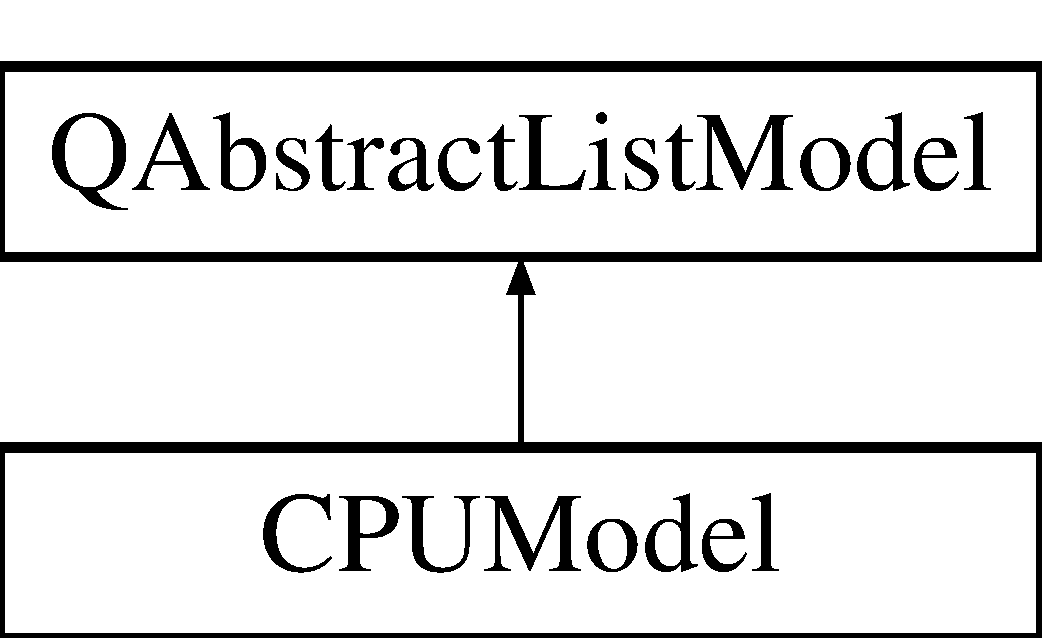
\includegraphics[height=2.000000cm]{class_c_p_u_model}
\end{center}
\end{figure}
\subsection*{Public Member Functions}
\begin{DoxyCompactItemize}
\item 
\hyperlink{class_c_p_u_model_aecf961723e84bc4d1782d2ecc2228e3d}{C\+P\+U\+Model} (Q\+Object $\ast$parent=0)
\item 
Q\+\_\+\+I\+N\+V\+O\+K\+A\+B\+LE void \hyperlink{class_c_p_u_model_a5d940e548d8e38476161a86f92a76aeb}{populate\+Model} ()
\item 
Q\+\_\+\+I\+N\+V\+O\+K\+A\+B\+LE Q\+String \hyperlink{class_c_p_u_model_a69b8398765d4e00e7394ddc1cf83b663}{pretty\+Format} (int index) const
\end{DoxyCompactItemize}


\subsection{Detailed Description}
The \hyperlink{class_c_p_u_model}{C\+P\+U\+Model} class This class contains the list model for processor information extracted from \textquotesingle{}/proc/cpuinfo\textquotesingle{} file in a Linux system. The class is derived from Q\+Abstract\+List\+Model. 

\subsection{Constructor \& Destructor Documentation}
\mbox{\Hypertarget{class_c_p_u_model_aecf961723e84bc4d1782d2ecc2228e3d}\label{class_c_p_u_model_aecf961723e84bc4d1782d2ecc2228e3d}} 
\index{C\+P\+U\+Model@{C\+P\+U\+Model}!C\+P\+U\+Model@{C\+P\+U\+Model}}
\index{C\+P\+U\+Model@{C\+P\+U\+Model}!C\+P\+U\+Model@{C\+P\+U\+Model}}
\subsubsection{\texorpdfstring{C\+P\+U\+Model()}{CPUModel()}}
{\footnotesize\ttfamily C\+P\+U\+Model\+::\+C\+P\+U\+Model (\begin{DoxyParamCaption}\item[{Q\+Object $\ast$}]{parent = {\ttfamily 0} }\end{DoxyParamCaption})}



\subsection{Member Function Documentation}
\mbox{\Hypertarget{class_c_p_u_model_a5d940e548d8e38476161a86f92a76aeb}\label{class_c_p_u_model_a5d940e548d8e38476161a86f92a76aeb}} 
\index{C\+P\+U\+Model@{C\+P\+U\+Model}!populate\+Model@{populate\+Model}}
\index{populate\+Model@{populate\+Model}!C\+P\+U\+Model@{C\+P\+U\+Model}}
\subsubsection{\texorpdfstring{populate\+Model()}{populateModel()}}
{\footnotesize\ttfamily void C\+P\+U\+Model\+::populate\+Model (\begin{DoxyParamCaption}{ }\end{DoxyParamCaption})}

populates model from cpuinfo file \mbox{\Hypertarget{class_c_p_u_model_a69b8398765d4e00e7394ddc1cf83b663}\label{class_c_p_u_model_a69b8398765d4e00e7394ddc1cf83b663}} 
\index{C\+P\+U\+Model@{C\+P\+U\+Model}!pretty\+Format@{pretty\+Format}}
\index{pretty\+Format@{pretty\+Format}!C\+P\+U\+Model@{C\+P\+U\+Model}}
\subsubsection{\texorpdfstring{pretty\+Format()}{prettyFormat()}}
{\footnotesize\ttfamily Q\+String C\+P\+U\+Model\+::pretty\+Format (\begin{DoxyParamCaption}\item[{int}]{index }\end{DoxyParamCaption}) const}

returns a complete string for a given index as key\+:value pairs @ index index of the list containing the key\+:value pairs 

The documentation for this class was generated from the following files\+:\begin{DoxyCompactItemize}
\item 
C\+:/\+Users/\+S\+H\+E\+K\+H\+A\+R/\+Desktop/\+C\+P\+U\+\_\+\+Info/cpu\+Information/\hyperlink{cpumodel_8h}{cpumodel.\+h}\item 
C\+:/\+Users/\+S\+H\+E\+K\+H\+A\+R/\+Desktop/\+C\+P\+U\+\_\+\+Info/cpu\+Information/\hyperlink{cpumodel_8cpp}{cpumodel.\+cpp}\end{DoxyCompactItemize}

\chapter{File Documentation}
\hypertarget{cpumodel_8cpp}{}\section{C\+:/\+Users/\+S\+H\+E\+K\+H\+A\+R/\+Desktop/\+C\+P\+U\+\_\+\+Info/cpu\+Information/cpumodel.cpp File Reference}
\label{cpumodel_8cpp}\index{C\+:/\+Users/\+S\+H\+E\+K\+H\+A\+R/\+Desktop/\+C\+P\+U\+\_\+\+Info/cpu\+Information/cpumodel.\+cpp@{C\+:/\+Users/\+S\+H\+E\+K\+H\+A\+R/\+Desktop/\+C\+P\+U\+\_\+\+Info/cpu\+Information/cpumodel.\+cpp}}
{\ttfamily \#include \char`\"{}cpumodel.\+h\char`\"{}}\newline
{\ttfamily \#include \char`\"{}globalconstants.\+h\char`\"{}}\newline
{\ttfamily \#include $<$Q\+File$>$}\newline
{\ttfamily \#include $<$Q\+Text\+Stream$>$}\newline
{\ttfamily \#include $<$Q\+Debug$>$}\newline

\hypertarget{cpumodel_8h}{}\section{C\+:/\+Users/\+S\+H\+E\+K\+H\+A\+R/\+Desktop/\+C\+P\+U\+\_\+\+Info/cpu\+Information/cpumodel.h File Reference}
\label{cpumodel_8h}\index{C\+:/\+Users/\+S\+H\+E\+K\+H\+A\+R/\+Desktop/\+C\+P\+U\+\_\+\+Info/cpu\+Information/cpumodel.\+h@{C\+:/\+Users/\+S\+H\+E\+K\+H\+A\+R/\+Desktop/\+C\+P\+U\+\_\+\+Info/cpu\+Information/cpumodel.\+h}}
{\ttfamily \#include $<$Q\+Abstract\+List\+Model$>$}\newline
{\ttfamily \#include $<$Q\+String\+List$>$}\newline
\subsection*{Classes}
\begin{DoxyCompactItemize}
\item 
class \hyperlink{class_c_p_u_model}{C\+P\+U\+Model}
\begin{DoxyCompactList}\small\item\em The \hyperlink{class_c_p_u_model}{C\+P\+U\+Model} class This class contains the list model for processor information extracted from \textquotesingle{}/proc/cpuinfo\textquotesingle{} file in a Linux system. The class is derived from Q\+Abstract\+List\+Model. \end{DoxyCompactList}\end{DoxyCompactItemize}

\hypertarget{globalconstants_8h}{}\section{C\+:/\+Users/\+S\+H\+E\+K\+H\+A\+R/\+Desktop/\+C\+P\+U\+\_\+\+Info/cpu\+Information/globalconstants.h File Reference}
\label{globalconstants_8h}\index{C\+:/\+Users/\+S\+H\+E\+K\+H\+A\+R/\+Desktop/\+C\+P\+U\+\_\+\+Info/cpu\+Information/globalconstants.\+h@{C\+:/\+Users/\+S\+H\+E\+K\+H\+A\+R/\+Desktop/\+C\+P\+U\+\_\+\+Info/cpu\+Information/globalconstants.\+h}}
\subsection*{Macros}
\begin{DoxyCompactItemize}
\item 
\#define \hyperlink{globalconstants_8h_a877b51b5856b94467bdd52f26e0729ec}{P\+R\+O\+C\+E\+S\+S\+O\+R\+\_\+\+T\+AG}~\char`\"{}processor\char`\"{}
\item 
\#define \hyperlink{globalconstants_8h_a1f899c6ab102bd5f2784b6de2116d0ae}{C\+P\+U\+I\+N\+F\+O\+\_\+\+F\+I\+LE}~\char`\"{}/proc/cpuinfo\char`\"{}
\end{DoxyCompactItemize}


\subsection{Macro Definition Documentation}
\mbox{\Hypertarget{globalconstants_8h_a1f899c6ab102bd5f2784b6de2116d0ae}\label{globalconstants_8h_a1f899c6ab102bd5f2784b6de2116d0ae}} 
\index{globalconstants.\+h@{globalconstants.\+h}!C\+P\+U\+I\+N\+F\+O\+\_\+\+F\+I\+LE@{C\+P\+U\+I\+N\+F\+O\+\_\+\+F\+I\+LE}}
\index{C\+P\+U\+I\+N\+F\+O\+\_\+\+F\+I\+LE@{C\+P\+U\+I\+N\+F\+O\+\_\+\+F\+I\+LE}!globalconstants.\+h@{globalconstants.\+h}}
\subsubsection{\texorpdfstring{C\+P\+U\+I\+N\+F\+O\+\_\+\+F\+I\+LE}{CPUINFO\_FILE}}
{\footnotesize\ttfamily \#define C\+P\+U\+I\+N\+F\+O\+\_\+\+F\+I\+LE~\char`\"{}/proc/cpuinfo\char`\"{}}

\mbox{\Hypertarget{globalconstants_8h_a877b51b5856b94467bdd52f26e0729ec}\label{globalconstants_8h_a877b51b5856b94467bdd52f26e0729ec}} 
\index{globalconstants.\+h@{globalconstants.\+h}!P\+R\+O\+C\+E\+S\+S\+O\+R\+\_\+\+T\+AG@{P\+R\+O\+C\+E\+S\+S\+O\+R\+\_\+\+T\+AG}}
\index{P\+R\+O\+C\+E\+S\+S\+O\+R\+\_\+\+T\+AG@{P\+R\+O\+C\+E\+S\+S\+O\+R\+\_\+\+T\+AG}!globalconstants.\+h@{globalconstants.\+h}}
\subsubsection{\texorpdfstring{P\+R\+O\+C\+E\+S\+S\+O\+R\+\_\+\+T\+AG}{PROCESSOR\_TAG}}
{\footnotesize\ttfamily \#define P\+R\+O\+C\+E\+S\+S\+O\+R\+\_\+\+T\+AG~\char`\"{}processor\char`\"{}}


\hypertarget{main_8cpp}{}\section{C\+:/\+Users/\+S\+H\+E\+K\+H\+A\+R/\+Desktop/\+C\+P\+U\+\_\+\+Info/cpu\+Information/main.cpp File Reference}
\label{main_8cpp}\index{C\+:/\+Users/\+S\+H\+E\+K\+H\+A\+R/\+Desktop/\+C\+P\+U\+\_\+\+Info/cpu\+Information/main.\+cpp@{C\+:/\+Users/\+S\+H\+E\+K\+H\+A\+R/\+Desktop/\+C\+P\+U\+\_\+\+Info/cpu\+Information/main.\+cpp}}
{\ttfamily \#include $<$Q\+Gui\+Application$>$}\newline
{\ttfamily \#include $<$Q\+Qml\+Application\+Engine$>$}\newline
{\ttfamily \#include $<$Q\+Quick\+View$>$}\newline
{\ttfamily \#include $<$Q\+Qml\+Context$>$}\newline
{\ttfamily \#include \char`\"{}cpumodel.\+h\char`\"{}}\newline
\subsection*{Functions}
\begin{DoxyCompactItemize}
\item 
int \hyperlink{main_8cpp_a0ddf1224851353fc92bfbff6f499fa97}{main} (int argc, char $\ast$argv\mbox{[}$\,$\mbox{]})
\end{DoxyCompactItemize}


\subsection{Function Documentation}
\mbox{\Hypertarget{main_8cpp_a0ddf1224851353fc92bfbff6f499fa97}\label{main_8cpp_a0ddf1224851353fc92bfbff6f499fa97}} 
\index{main.\+cpp@{main.\+cpp}!main@{main}}
\index{main@{main}!main.\+cpp@{main.\+cpp}}
\subsubsection{\texorpdfstring{main()}{main()}}
{\footnotesize\ttfamily int main (\begin{DoxyParamCaption}\item[{int}]{argc,  }\item[{char $\ast$}]{argv\mbox{[}$\,$\mbox{]} }\end{DoxyParamCaption})}


%--- End generated contents ---

% Index
\backmatter
\newpage
\phantomsection
\clearemptydoublepage
\addcontentsline{toc}{chapter}{Index}
\printindex

\end{document}
